% Created 2011-01-05 Ср. 20:58
\documentclass[12pt, russian, oneside, article]{ncc}
\usepackage[utf8]{inputenc}
\usepackage[T1]{fontenc}
\usepackage{fixltx2e}
\usepackage{graphicx}
\usepackage{longtable}
\usepackage{float}
\usepackage{wrapfig}
\usepackage{soul}
\usepackage{textcomp}
\usepackage{marvosym}
\usepackage{wasysym}
\usepackage{latexsym}
\usepackage{amssymb}
\usepackage{hyperref}
\tolerance=1000
\usepackage[math]{pscyr}
\usepackage{indentfirst}
\providecommand{\alert}[1]{\textbf{#1}}
\begin{document}



\title{Теория систем}
\author{Максим Захаров}
\date{05 Январь 2011}
\maketitle

\setcounter{tocdepth}{3}
\tableofcontents
\vspace*{1cm}

\href{file://~/Documents/Git/lectures/other~/Documents/Git/zamal.github.com/pdf/TS_Lectures.pdf}{Скачать в PDF}

\section{Лекция 1 <2010-09-02 Чтв>}
\label{sec-1}


Главное отличие естественных систем от искусственных -- ``известность'' цели функционирования.

Искусственные системы делятся:
\begin{enumerate}
\item С управлением.
\item Без управления.
\end{enumerate}

Под управлением понимается процесс формирования целенаправленного поведения системы посредством информационных воздействий. Информационные воздействия могут вырабатываться человеком или устройством.   
  
Задачи управления:
\begin{enumerate}
\item Задача целеполагания. Определение требуемого состояния и поведения системы.
\item Задача стабилизации. Удержание системы в существующем состоянии в условиях возмущающих воздействий.
\item Выполнение программы. Перевод системы в требуемое состояние в условиях, когда значения управляемых величин изменяются по известным детерминированным законам.
\item Задача слежения. Удержание системы на заданной траектории в условиях, когда законы изменения управляемых величин неизвестны или изменяются.
\item Задача оптимизации. Удержание и перевод системы в состояние с экстремальными значениями характеристик при заданных условиях или ограничениях.
\end{enumerate}
\section{Лекция 2 <2010-09-09 Чтв>}
\label{sec-2}


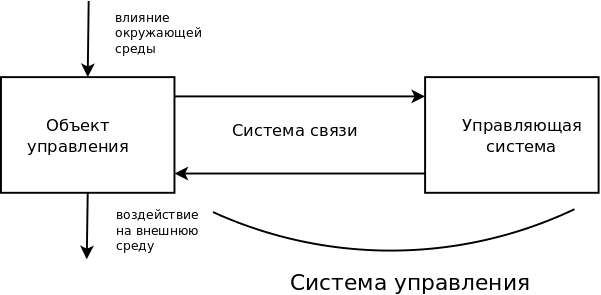
\includegraphics[width=0.5\textwidth]{images/TS/sistema.png}

Индивидуум или группа индивидуумов, имеющих право принимать окончательное решение по выбору одно из нескольких управляющих воздействий, называется лицом, принимающим решения (ЛПР).

Функции системы управления:
\begin{enumerate}
\item Коммуникационная (обмена информацией).
\item Рутинные функции обработки информации.
\item Принятия решения.
\end{enumerate}
\section{Лекция 3 <2010-09-16 Чтв>}
\label{sec-3}


Пути совершенствования систем с управлением:
\begin{enumerate}
\item Оптимизация численности управленческого персонала.
\item Использование новых способов организации системы управления.
\item Применение новых методов решения управленческих задач.
\item Изменение структуры системы управления.
\item Перераспределение функций, задач в системе управления.
\item Механизация управленческого труда.
\item Автоматизация.
\end{enumerate}

Цели автоматизации управления:
\begin{enumerate}
\item Уменьшить время принятия решений.
\item Улучшить качество принимаемых решений.
\end{enumerate}

Эти цели достигаются путями:
\begin{enumerate}
\item Повышение оперативности управления.
\item Снижение трудозатрат ЛПР.
\item Повышение степени обоснованности принятых решений.
\end{enumerate}
\section{Лекция 4. <2010-09-23 Чтв>}
\label{sec-4}


\emph{Системный анализ} --- это методология решения проблем, основанная на структуризации систем и количественном сравнении альтернатив.

Основные задачи:
\begin{enumerate}
\item Декомпозиция. Это представление системы в виде подсистем, состоящих из более мелких элементов.
\item Анализ. Она состоит в нахождении свойств системы или свойств среды, окружающую систему.
\item Синтез. Состоит в том, что по описанию закона преобразования необходимо реализовать алгоритм. При решении задачи синтеза часто решается задача оптимизации --- выбор из нескольких альтернатив оптимального.

\begin{itemize}
\item однокритериальная;
\item многокритериальная.
\end{itemize}

\end{enumerate}

Классификация систем:
\begin{enumerate}
\item Физическая.
\item Абстрактная.
\end{enumerate}

Системы делятся на:
\begin{enumerate}
\item Простые.
\item Сложные:

\begin{itemize}
\item робастность. Способность сохранять полную или частичную работоспособность при отказе некоторых элементов;
\item эмерджентность (интегративность, целостность). Свойства системы большее, чем совокупность свойств, составляющих её элементы;
\item наличие большого числа разнообразных разнородных связей между элементами

\begin{itemize}
\item структурные;
\item функциональные;
\item казуальные;
\item информационные;
\item пространственно-временные.
\end{itemize}

\end{itemize}

\end{enumerate}
\section{Лекция 5. <2010-09-30 Чтв>}
\label{sec-5}


Системы могут быть:
\begin{enumerate}
\item Естественные.
\item Искусственные.
\end{enumerate}

$x(t)$ --- множество функций входных воздействий.

$y(t)$ --- множество выходных характеристик системы.

$z(t)$ --- множество состояний системы.

В зависимости от вида этих функций системы делят на:
\begin{enumerate}
\item Дискретные.
\item Непрерывные.
\end{enumerate}

Деление не дискретные и непрерывные происходит с точки зрения исследователя.


\begin{enumerate}
\item Стохастические. Функция входа может иметь случайные характер, или функция множества состояный носит случайный характер.
\item Детерминированные. Все состояния чётко определены.
\end{enumerate}
\begin{enumerate}
\item Открытые. Системы, в которых неоднозначность реакции на воздействие нельзя объяснить разницей состояний.
\item Закрытые.
\end{enumerate}
\section{Лекция 6. <2010-10-07 Чтв>}
\label{sec-6}
\subsection{Основные определения системного анализа}
\label{sec-6_1}


\emph{Элемент} --- некоторый объект, обладающий рядом важных свойств и реализующий в системе определённый закон функционирования, внутренняя структура которого не рассматривается.

На вход системы 3 воздействия:
\begin{enumerate}
\item Управляющие.
\item Неуправляемые.
\item Возмущающие.
\end{enumerate}

\emph{Среда} --- множество объектов, вне данной системы, которая оказывает влияние на систему и сами находятся под воздействием системы.

\emph{Подсистема} --- часть системы, выделенная по определённому признаку, обладающая некоторой самостоятельностью и допускающая разложения на элементы.

\emph{Характеристика} --- это, что отражает некоторые свойства системы.
Характеристика задаётся кортежом <имя, \{значения\}>.
\section{Лекция 7. <2010-10-14 Чт.>}
\label{sec-7}


Характеристики бывают количественные и качественные. Количественные характеристики называются параметрами.

Оптимизация может быть однокритериальной и многокритериальной.

Под свойством понимают то, что обуславливает отличие одного объекта от другого или наоборот сходство между ними и проявляющееся во взаимодействии с другими объектами. Характеристики системы отражают её свойства.

Свойства делят на внутренние и внешние. Внешние свойства можно наблюдать, они проявляются в виде характеристик системы. Внутренние свойства наблюдать нельзя, они проявляются в виде состояний системы. Внутренние свойства являются причиной внешние свойств.

При исследовании свойства задаются в виде отношений. Существует несколько форм представления отношений:
\begin{enumerate}
\item Функциональная.
\item Матричная или табличная.
\item Логические.
\item Графовые.
\item Представления сечениями.
\item Алгоритмическая.
\end{enumerate}

Одна из основных целей системного анализа --- выявление внутренних свойств системы, определяющих её поведение. По структуре делятся на простые и интегральные.

Внутренние свойства конструируются в нашем сознании логически и недоступны наблюдению.

Горизонтальные уровни анализа называются иерархическими. Вертикальные называются аспектами.
\section{Лекция 8. <2010-10-21 Чт.>}
\label{sec-8}


Закон функционирования описывает процесс функционирования элемента для всей системы в целом.

Закон функционирования
$y(t) = F(x, n, u, t)$
x - полезная нагрузка
n - мешающее воздействие
u - управляющее воздействие

Поведение системы во времени --- это изменение состояний системы.

Цель --- это ситуация или область ситуации, которая должна быть достигнута при функционировании системы за определённый промежуток времени.

Показатель --- характеристика, отражающая качества системы.
Показатели делятся на:
\begin{enumerate}
\item Частные показатели качества.
\item Обобщённые показатели качества.
\end{enumerate}

Кроме показателей качества есть показатели эффективности.

Различие между показателями качества и эффективности состоит в том, что показатель эффективности характеризует процесс (алгоритм) и эффект от функционирования системы, а показатели качества --- пригодность системы для использования по назначению.

Связь --- вид отношений между элементами системы, который проявляется в виде обмена. Связи делят на:
\begin{itemize}
\item внутренние --- между элементами;
\item внешние. Определение внешних связей позволяет выделить систему из среды.
\end{itemize}
\section{Лекция 9. <2010-10-28 Чтв>}
\label{sec-9}


Различают несколько видов связей:
\begin{enumerate}
\item Структурная. Задаются в графовой и матричной форме.

\begin{itemize}
\item иерархические;
\item сетевые;
\end{itemize}

\item Функциональные.
\item Пространственно-временные. Задаются как функции, функционалы и операторы.
\item Причинно-следственные. Описываются на языке формальной логики.
\item Информационные связи. В виде инфологической модели.
\end{enumerate}

Выделение связи позволяет судить о сложности системы.

Алгоритм функционирования --- метод получения выходных характеристик с учётом входных воздействий, управляющих, мешающих воздействий внешней среды.

Качество --- совокупность существенных свойств объекта, обуславливающих его использование по назначению. По одному интегральному свойству через один обобщённый показатель качества системы.

Процесс --- совокупность состояний системы, упорядоченная по изменению какого-либо параметра.

Совокупность всех возможных состояний называется пространством состояний.

Эффективность процесса --- степень его приспособленности к достижению цели.
\section{Практика}
\label{sec-10}


Можно выделить следующие типы виртуализации:
\begin{enumerate}
\item Программную виртуализацию:

\begin{itemize}
\item динамическая виртуализация;
\item паравиртуализация.
\end{itemize}

\item Аппаратную виртуализации.
\end{enumerate}

Гипервизоры:
\begin{enumerate}
\item Первого типа bare metal.

\begin{itemize}
\item Xen.
\item Hyper-V.
\item KVM.
\item VMWare ESX.
\end{itemize}

\item Второго типа (как задача в обычной ОС).

\begin{itemize}
\item MS Virtual PC 2007.
\item VirtualBox.
\item VMWare.
\item Parallels.

       GUEST
\end{itemize}

\end{enumerate}
H|    | 32 | 64 |
O|----+----+----|
S| 32 |  + |  В |
T| 64 |  В |  В |

В --- обязательная поддержка аппаратной виртуализации процессором.

\begin{enumerate}
\item NAT.
\item Мост.
\item Внутренняя сеть.
\item Хост адаптер.
\end{enumerate}

\end{document}
